\documentclass[12pt]{article}
\usepackage{amsmath, amssymb, amsbsy}
\usepackage{graphicx, subfigure,listings}
\usepackage[margin=1in,nohead]{geometry}
\usepackage{float}
\usepackage[style=ieee,natbib=true,backend=bibtex]{biblatex}
\setlength{\parindent}{0pt}
\setlength{\parskip}{12pt}
\bibliography{E296}
\lstdefinestyle{myCustomMatlabStyle}{
  language=Matlab,
  numbers=none,
  stepnumber=1,
  numbersep=10pt,
  tabsize=4,
  showspaces=false,
  showstringspaces=false
}
\lstset{basicstyle=\normalsize,style=myCustomMatlabStyle}

\begin{document}
\noindent E296MA\\ Dr. Gabriel Gomez \\ Fall 2017

\section*{MATLAB Tutorial 1 - Solving Linear Systems, Plotting and Visualization, and Objects}
MATLAB is a user-friendly computational tool used throughout academia and industry. It has countless powerful toolboxes, and allows the user to quickly write code to expedite mathematical computation. The advantage of MATLAB over other scientific computing software, such as Python, is the ease of use. For example, almost all the necessary software packages are built into MATLAB and rarely does the user need to load particular packages. This make computation fast and easy.

In this tutorial, we will go over: 

importing datalk about solutions to linear systems (i.e. linear equations that can be expressed in Matrix form), plotting and visualization, and finally, objects. 

\begin{enumerate}
\item Importing Data
\item Visualization (2D and 3D)
\item Curve fitting
\item Solving linear systems
\item Object Oriented Programming
\end{enumerate}

\section{Data Import, Visualization, Curve Fitting}

\subsection{Data Import and Visualization}
Import data from the internet by pasting the following into Matlab:

\begin{lstlisting}[frame=single]
api = 'http://climatedataapi.worldbank.org/climateweb/rest/v1/';
url = [api 'country/cru/tas/year/USA'];
S = webread(url);
\end{lstlisting}

This will load a structured array \lstinline|S| with information about the \lstinline|year| and the temperature \lstinline|data|. This data can be extracted with the following syntax

\begin{lstlisting}[frame=single]
years = [S.year];
temps = [S.data];
temps = 9/5 * temps + 32; %Convert to Fahrenheit
yearstoplot = datetime(years,1,1); %Convert years to 'datetime'
\end{lstlisting}

Note that the brackets are necessary with this type of structured array. Without the brackets you will only access the last data entry. The last two lines convert the temperature data to Fahrenheit and convert the year data to a standard datetime format that can be directly read by MATLAB.

To plot the data

\begin{lstlisting}[frame=single]
%Plot data 
figure
plot(yearstoplot, temps,'ok');
title('USA Average Temperature 1901-2012')
xlabel('Year')
ylabel('Temperature (^{\circ}F)')
xmin = yearstoplot(1);
xmax = yearstoplot(end);
xlim([xmin xmax])

\end{lstlisting}

\begin{figure}[H]
\centering
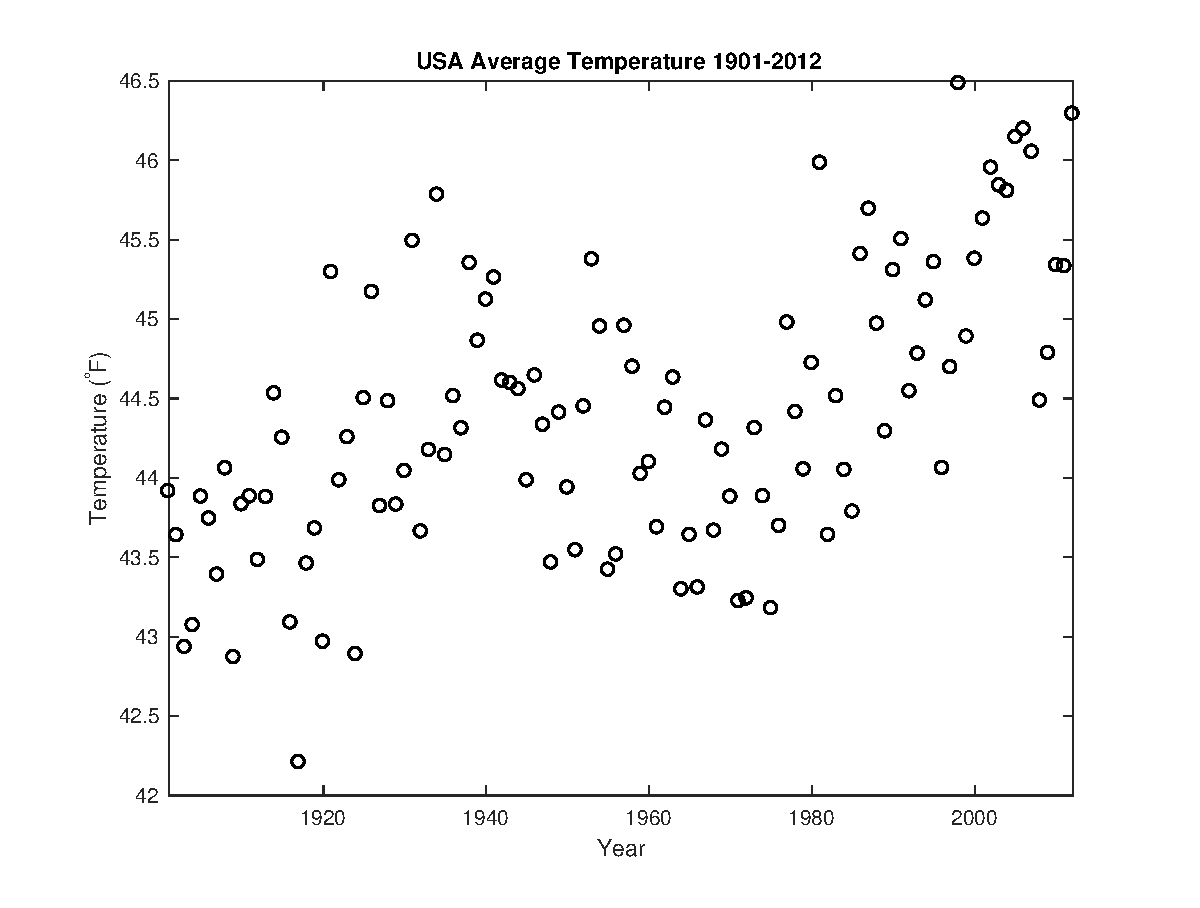
\includegraphics[width=0.75\linewidth]{tempVsYearAll.eps}
\end{figure}

\subsection{Split Data into Training and Test Set}
In order to text the prediction capabilities of a model, it is important to segment out two sets of data. The training data consists of the data that we will use to `train' our model. This is the data that we will fit a curve too. The other set of data is called the `test' data. This dataset is used to evaluate the predictive capability of our trained model. 

In our case we will split the data at the year 1990; everything before 1990 will be considered `training' data, and everything after 1990 will be considered `test' data. You can use the following code to segment the test and training data. 

\begin{lstlisting}[frame=single]
%% Split data into training set and test set
yearfortraintest=1990;

indices_train=years<=yearfortraintest;
years_train = years(indices_train);
temps_train = temps(indices_train);
yearstoplot_train=yearstoplot(indices_train);

indices_test=years>yearfortraintest;
years_test = years(indices_test);
temps_test = temps(indices_test);
yearstoplot_test=yearstoplot(indices_test);
\end{lstlisting}

\subsection{Curve Fitting on Training Data}
Now, we will fit a model to our training data. We will use different degree polynomials. The simplest polynomial is a line, i.e. y=mx+b. To fit a line to our data we can use the following code:

\begin{lstlisting}[frame=single]
%Fit 1-degree polynomial
[p1_all,~,mu1_all] = polyfit(years_train,temps_train,1);
p1temps_train = polyval(p1_all,years_train,[],mu1_all); %evaluate polynomial
hold on; xlim([yearstoplot_train(1) yearstoplot_train(end)]);
f1 = plot(yearstoplot_train, p1temps_train,'r'); 
xlim([yearstoplot_train(1) yearstoplot_train(end)]);
R_squared_train1=1-sum((p1temps_train-temps_train).^2)/...
    (((length(temps_train)-1) * var(temps_train)))
norm2_train1=norm(p1temps_train-temps_train,2)
\end{lstlisting}

There is also a nice interface for curve fitting in Matlab, called \lstinline|cftool|. This is a user friendly interface that lets you easily fit data to a user-specified function. Try it out by typing   \lstinline|cftool| into the command line. 

\begin{enumerate}
\item[Try:] Use either polyfit or \lstinline|cftool| to fit 2nd and 3rd degree polynomial to the training data. Try the \lstinline|center and scale| option to find a better conditioned polynomial.  Plot all three polynomials on the same axis. 
\item[Try:] Obtain the R-squared value of each polynomial
\item[Try:] Obtain the 2-norm value of each fitted function. The 2-norm (a.k.a. Euclidean Norm) of a vector $x_i = f_i-y_i$  is $||x||_2=\sqrt{\sum_i(x_i)^2}$. 
\end{enumerate}

You should end up with a plot that looks like the following:

\begin{figure}[H]
\centering
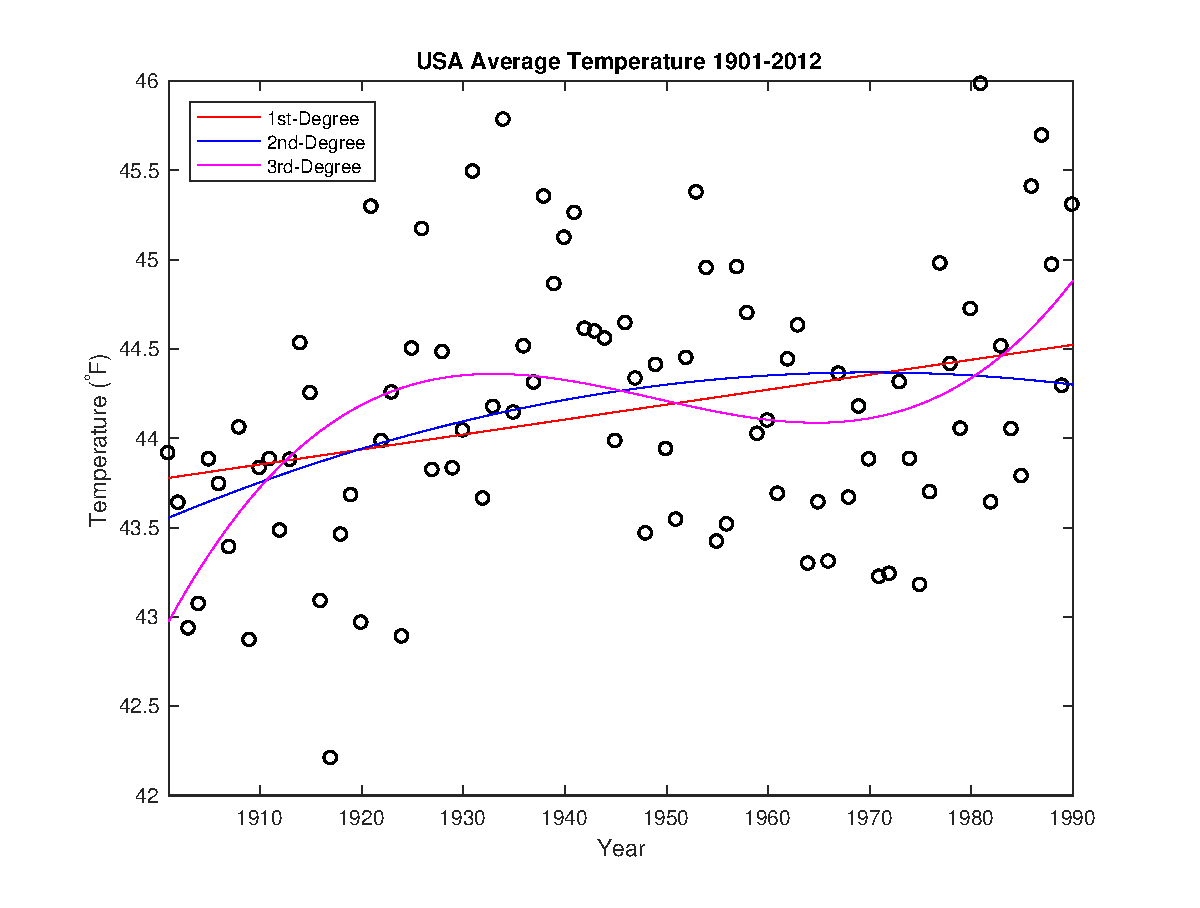
\includegraphics[width=0.75\linewidth]{tempVsYearTrain.eps}
\end{figure}

\begin{enumerate}
\item[Q:] Which function do you think best describes the data? Why?
\end{enumerate}

\subsection{Prediction}
To evaluate which curve best describes the data, we need to think about not just how well the curve describes previous data, but how well the curve describes as of yet unknown data. To do this, we split our data into training and test sets, pretending that we do not know what happens after the year 1990. Now, we use the test data to evaluate how well predictions based on our curve fits describe what happens in the period from 1991-2012. 

To do this, we evaluate our polynomials for years 1991-2012, and compare to the actual measured data. This can be done using the following code

\begin{lstlisting}[frame=single]
%test 1-degree polynomial
p1temps_test = polyval(p1,years_test,[],mu1); %evaluate polynomial
hold on; xlim([yearstoplot(1) yearstoplot(end)]);
f1 = plot(yearstoplot_test, p1temps_test,'r-*');
norm2_test1=norm(p1temps_test-temps_test,2)
\end{lstlisting}

We have also calculated the 2-norm to evaluate how well our predictions describe the test data. 

\begin{enumerate}
\item[Try:] Calculate predictions in the 1991-2012 period using the 2nd and 3rd degree polynomial to the training data. Plot all three polynomials on the same axis. 
\item[Try:] Obtain the 2-norm value of each fitted function. The 2-norm (a.k.a. Euclidean Norm) of a vector $x_i = f_i-y_i$  is $||x||_2=\sqrt{\sum_i(x_i)^2}$. 
\end{enumerate}

Now you end up with a figure that looks like the following:

\begin{figure}[H]
\centering
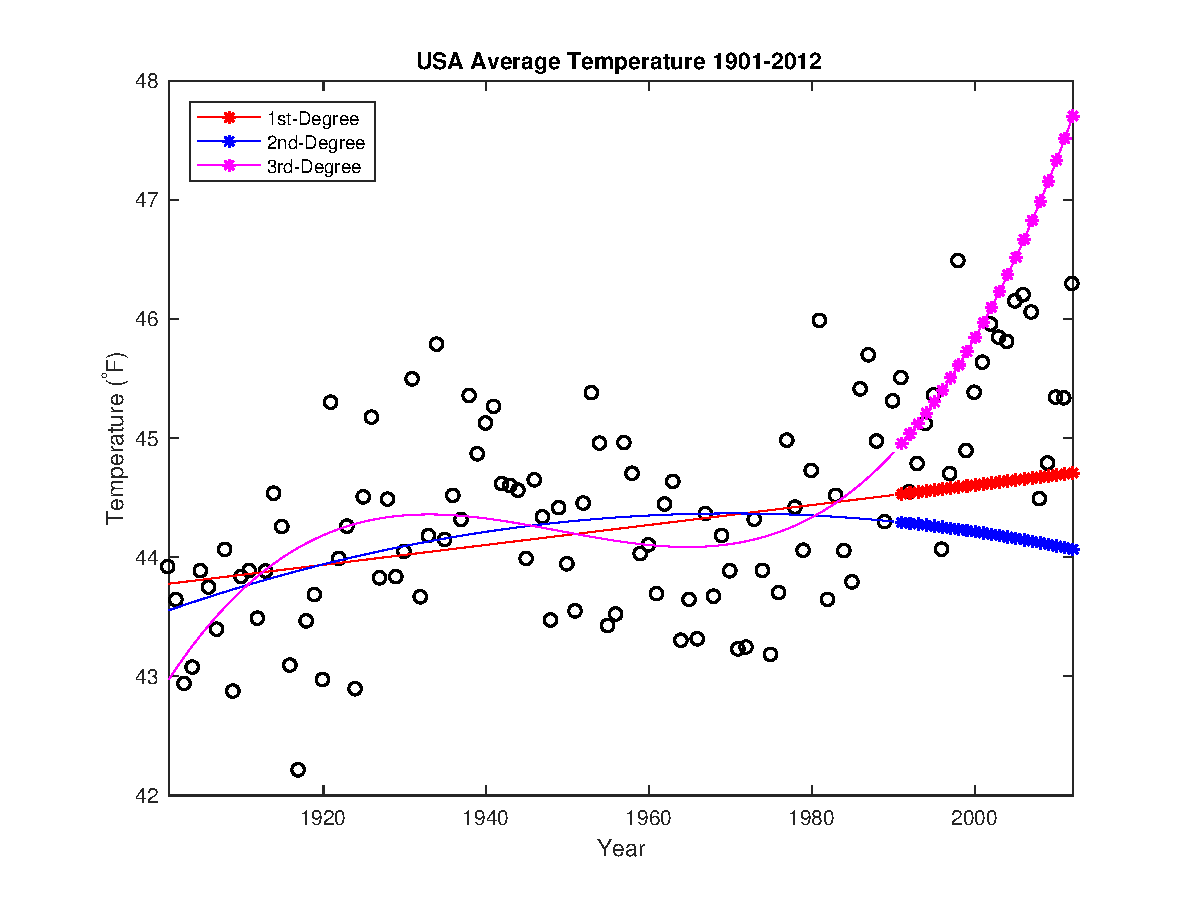
\includegraphics[width=0.75\linewidth]{tempVsYearTest.eps}
\end{figure}

\begin{enumerate}
\item[Q:] Now, which function do you think best describes the data? Why?
\end{enumerate}

\subsection{Homework}
Perform a curve fit on the entire dataset (years 1901-2012) for the 1st, 2nd, and 3rd degree polynomial. For each of the three functions, extrapolate predictions from 2013 to 2050. Plot the three predictions and comment on which function you believe gives the most realistic predictions for the period 2012-2050. Turn in with Homework set 3. 

\newpage

\section{Gaussian Distributions}

In this section we will go over statistical models. Specifically, we will go over how to use data to define a Gaussian distribution in MATLAB. The dataset we will use is measurements of height and weight of 25000 subjects in Hong Kong\cite{leung_weight-for-age_1996}. 

\subsection{Data Import}

This time we will import data from a .mat file that was previously created and saved. Ensure that the .mat file is in your current directory. 

\begin{lstlisting}[frame=single]
load humandata25000.mat
index=data(:,1);    %subject index
height=data(:,2);   %inches 
weight=data(:,3);   %pounds
\end{lstlisting}

Once the data has been imported, we can plot and visualize it wit the following commands

\begin{lstlisting}[frame=single]
plot(height,weight,'o'); hold on;
title('Weight vs. Height')
xlabel('Height (in)'); ylabel('Weight (kg)');
\end{lstlisting}

You should end up with a plot that looks like

\begin{figure}[H]
\centering
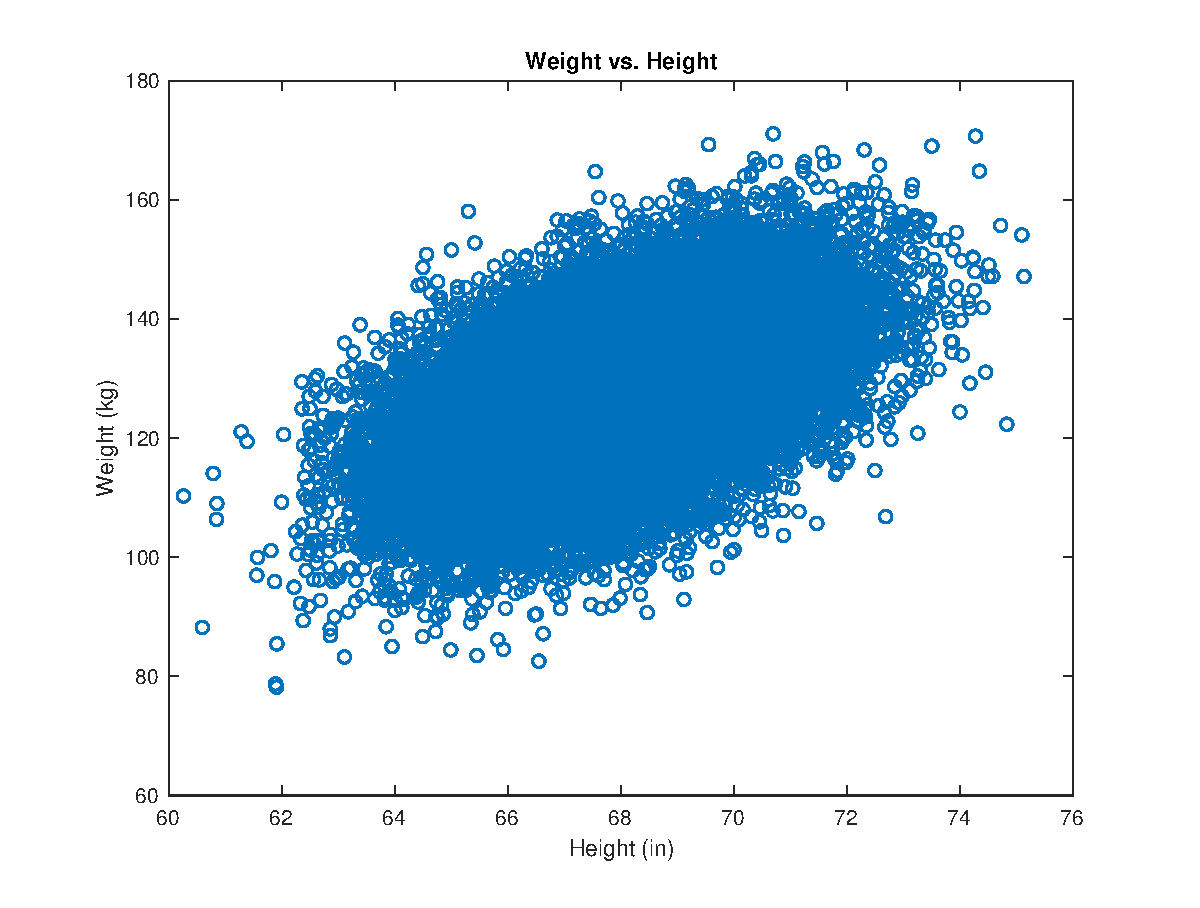
\includegraphics[width=0.75\linewidth]{plotHeightWeight.eps}
\end{figure}

\subsection{Random Sampling}
We now take random samples from our large dataset of 25000 subjects to develop progressively more accurate distributions of the population. Using the code below, we can draw four histograms created with samples of 5, 10, 100, and the entire dataset of 25000. Also, log the mean of each of these samples for later use. 

\begin{lstlisting}[frame=single]
%% Random Sampling of Gaussian - Heights
samples=[5,10,100,25000];
xlimits_height=[min(height),max(height)];
figure(1);
randsamples=randi([min(index) max(index)],samples(1),1);
subplot(5,1,1); h25=histogram(height(randsamples),10);
title(sprintf('Histogram %d Samples', samples(1)))
ylabel('Frequency')
xlim(xlimits_height)

randsamples=randi([min(index) max(index)],samples(2),1);
subplot(5,1,2); h250=histogram(height(randsamples),10);
title(sprintf('Histogram %d Samples', samples(2)))
ylabel('Frequency')
xlim(xlimits_height)

randsamples=randi([min(index) max(index)],samples(3),1);
subplot(5,1,3); h2500=histogram(height(randsamples),25);
title(sprintf('Histogram %d Samples', samples(3)))
ylabel('Frequency')
xlim(xlimits_height)

randsamples=randi([min(index) max(index)],samples(4),1);
subplot(5,1,4); h25000=histogram(height(randsamples),50);
title(sprintf('Histogram %d Samples', samples(4)))
ylabel('Frequency')
xlim(xlimits_height)
\end{lstlisting}

You'll end up with plots that look like the top four of the figure below. 

\subsection{Fitting a Gaussian to Data}
We now wish to describe the height distribution with a continuous Gaussian distribution. We do this by defining a probability density function (pdf) based on all 25000 subjects. This is done with the following

\begin{lstlisting}[frame=single]
%% fit gaussian to data
pd_height = fitdist(height,'Normal');
prob_height=pdf(pd_height,xlimits_height(1):0.1:xlimits_height(2));
subplot(5,1,5); plot(xlimits_height(1):0.1:xlimits_height(2),prob_height)
title('Probability Distribution Function')
ylabel('Probability')
xlabel('Height [in]')
xlim(xlimits_height)
\end{lstlisting}

The fitted gaussian is plotted in the 5th frame of the figure below. 

\begin{figure}[H]
\centering
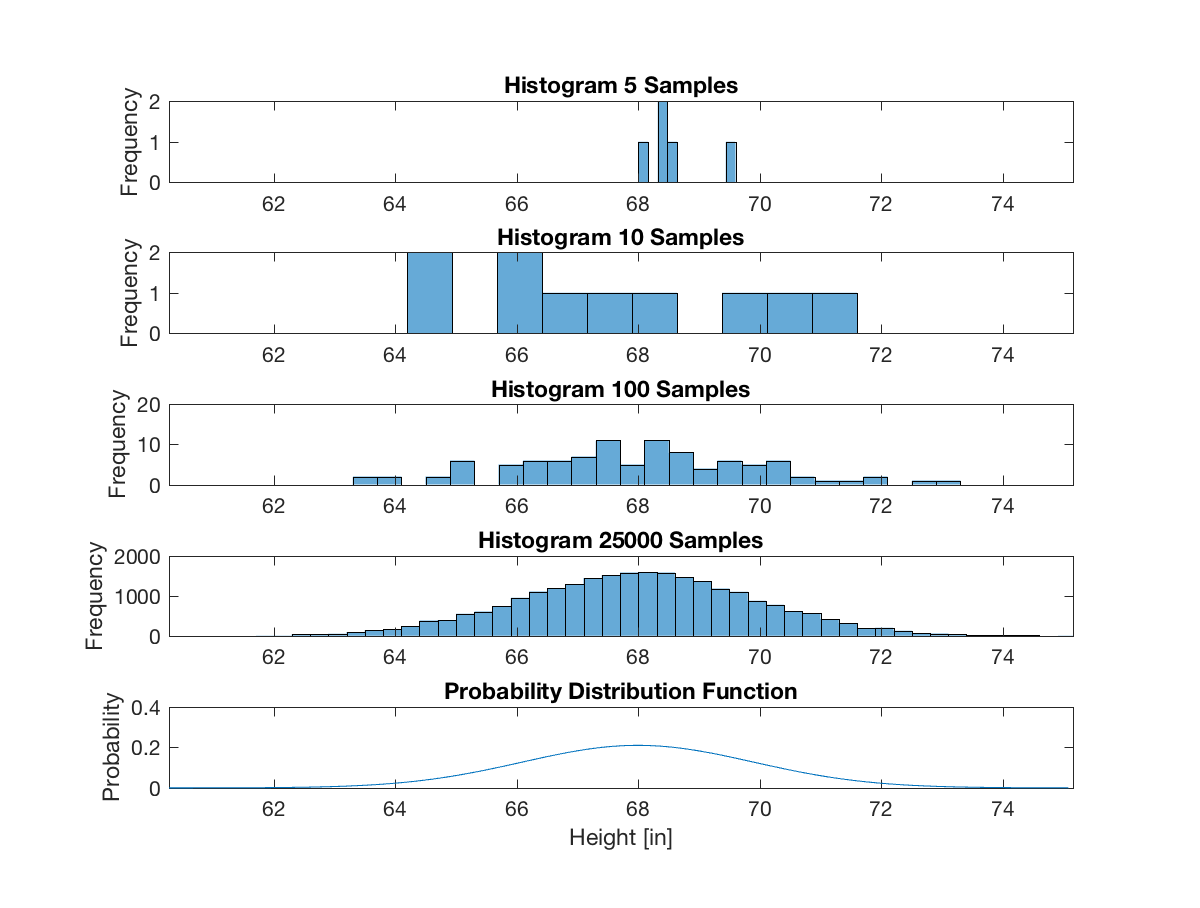
\includegraphics[width=0.75\linewidth]{heightHistograms.eps}
\end{figure}

\subsection{Law of Large Numbers}

The law of large numbers postulates that as the number of samples of a population increases, the mean will approach the theoretical mean of the population. To demonstrate this we will take random samples of size $N$ from our PDF. We take the mean of each of these samplings and plot the mean vs. sample size. This can be done with the following code

\begin{lstlisting}[frame=single]
figure(2);
%calculate the mean of N random samples taken from the pd
N=1:10:10000;
for i = 1:length(N)
    samplemean(i)=mean(random(pd_height,[N(i),1]));
end
semilogx(N,samplemean);
title('Sample Mean vs. Number of Samples')
xlabel('Number of Samples')
ylabel('Mean')
meanline=refline([0 pd_height.mu]);
meanline.LineStyle='--';
\end{lstlisting}

Your plot will show that as the sample size increases, the mean converges to the population mean, shown by the dotted line. Note that in our case we have assumed the population mean is equivalent to the mean of the PDF.

\begin{figure}[H]
\centering
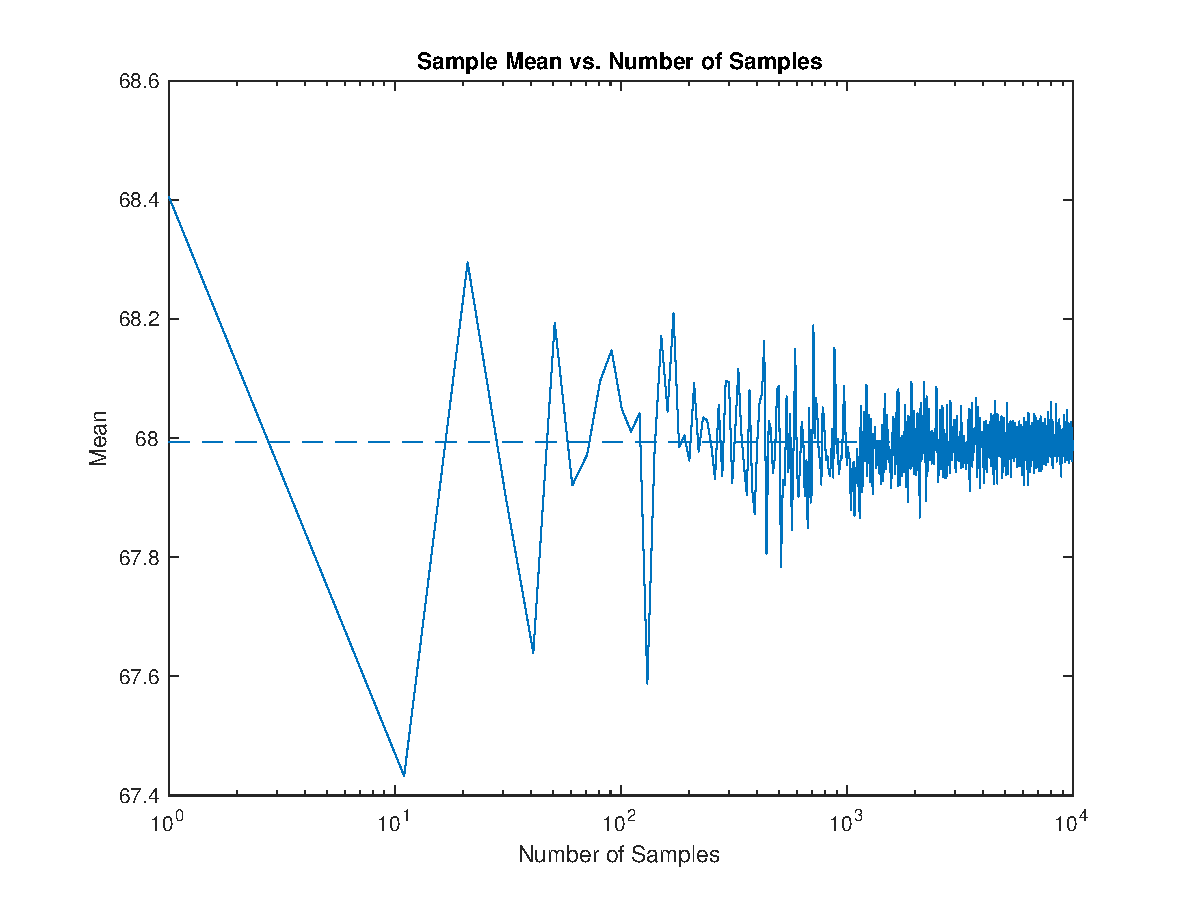
\includegraphics[width=0.75\linewidth]{plotLawLargeNum.eps}
\end{figure}

\subsection{3D Plotting - Histograms}

Although we have focused on the height data, the weight data is also of interest. To visualize the relationship between height and weight, we create a 3D histogram using the following code

\begin{lstlisting}[frame=single]
%% 3D Histogram
figure;
[a,b]=hist3([height,weight],[50,50]);
surf(b{1},b{2},a); shading interp; axis tight
title('3D Histogram')
xlabel('Height (in)'); ylabel('Weight (kg)'); zlabel('frequency')
\end{lstlisting}

\begin{figure}[H]
\centering
\includegraphics[width=0.75\linewidth]{surfHeightWeight.eps}
\end{figure}

If we visualize the 3D histogram from the top, it is evident that there is a strong relationship between weight and height. This 3D histogram is another representation of the data depicted in the first figure, which shows a scatter plot of height and weight. 

\subsection{Matrix Inversion and Linear Regression}

If we wish to find the linear relationship between weight and height, we can carry out a linear regression. This can be done as in the first part of this tutorial using \lstinline|polyfit|, however to demonstrate matrix inversion, we will find the best fit line using matrices. 

First, in general a line (or plane in 3D, or hyperplane in multiple dimensions) can be described by the matrix system
\begin{align*}
Ax=y.
\end{align*}

In this case, vector $x$ can be thought of as the `coefficients' of the line. We can solve for these coefficients by inverting matrix $A$ we can solve for $x$ 
\begin{align*}
x=A^{-1}y.
\end{align*}

Generally, a matrix must be square to find its inverse. However, in many cases $A$ will not be square. When $A$ is not square we can find what is called its `pseudoinverse' $A^{+}$. This can be found by multiplying $Ax=y$ by $A^{T}$. Because $A^{T}A$ is a square matrix, it is invertable 
\begin{align*}
Ax&=y\\
A^{T}Ax&=A^{T}y\\
x&=(A^{T}A)^{-1}A^{T}y\\
x&=A^{+}y.
\end{align*}

Finding the pseudoinverse is akin to finding the best fit solution to an over or underdefined system (no unique solutions vs. many unique solutions).

The rigorous, the mathematical theory behind the pseudoinverse is beyond the scope of this class. The thing worth remembering is that finding the inverse of a non-square matrix is analogous to finding the best fit solution to the system, and is equivalent to linear-regression.  

Now we will use MATLAB to find the pseudoinverse of A. Note that the `backslash \textbackslash' operator, which we will use will automatically decide if the matrix is square, under, or overdefined, and will calculate either the regular inverse or pseudoinverse accordingly. 

To make our matrix system specific to our problem we define $A$ as a N by 2 matrix that contains the known height data and a column of 1s, called $[1]$. The column of 1s allows us to add a constant coefficient to our vector $x$. This is equivalent to adding a y-intercept to the equation of a line: $y(:)=A(:,1)\cdot x(1)+1 \cdot x(2)$, because $(A(:,2)=[1])$. Last we define $y$ as an N by 1 vector that contains the weight data.
\begin{align*}
A&=[height_{data}, [1]]\\
x&=[x(1); x(2)]\\
y&=[weight_{data}]
\end{align*}

To solve for our coefficient vector $x$ we invert $A$ and multiply by $y$. This can be done using the following code, which calculates the pseudoinverse using the `backslash \textbackslash' operator

\begin{lstlisting}[frame=single]
%A*x=y or height*x=weight. To solve for x, we invert
A=[height,ones(size(height))]; %N by 2 matrix
y=[weight]; %N by 1 vector
x=A\y; %this is the matrix inversion step. In this case we are calculating the 'pseudo-inverse'.
y_pred=polyval(x,height);
plot(height,y_pred)
legend('data','Linear Fit')
\end{lstlisting}

The resulting line, looks like

\begin{figure}[H]
\centering
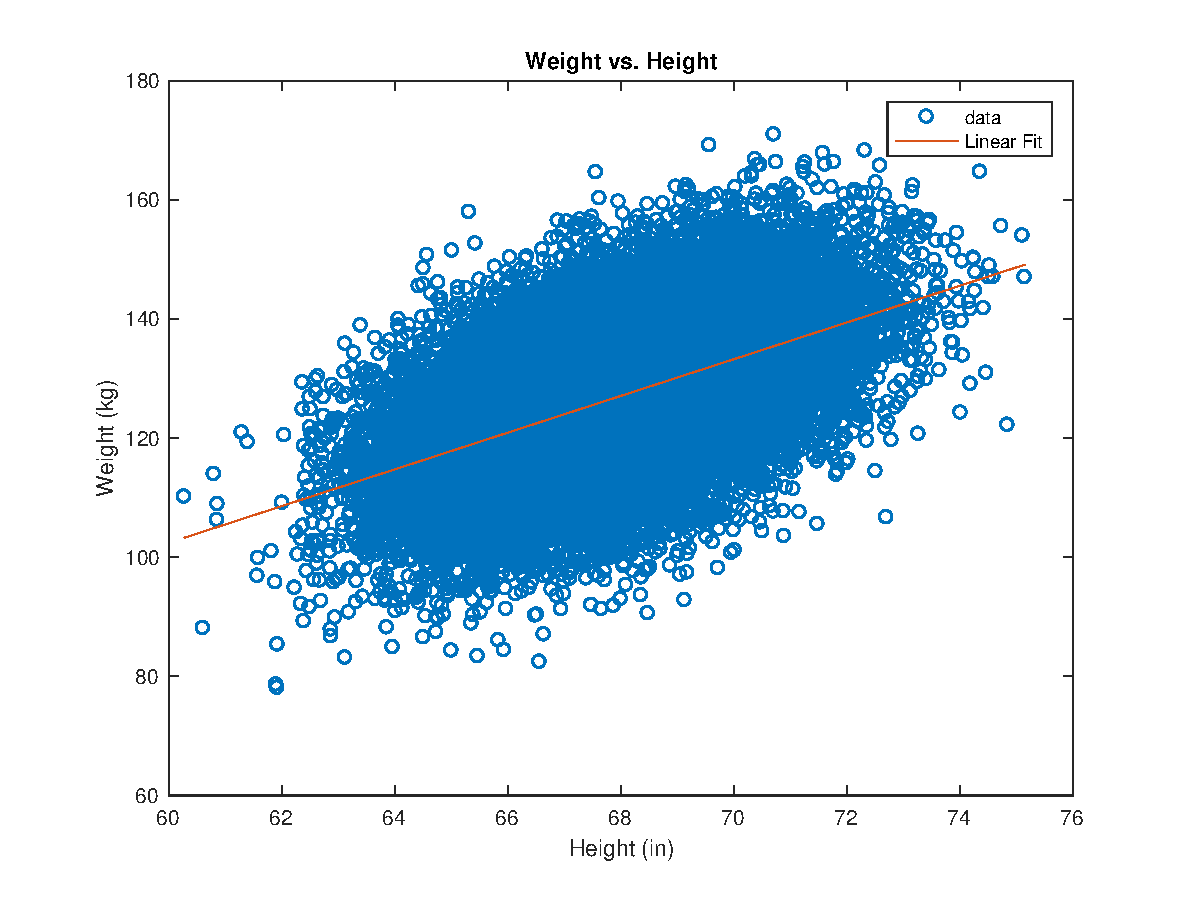
\includegraphics[width=0.75\linewidth]{linearFitHeightWeight.eps}
\end{figure}

\subsection{Homework}
Using the weight data (instead of height) create the four histograms, fit a gaussian distribution, and plot the sample mean vs. sample size (law of large numbers). Your figures should be similar to the height histogram and mean height vs. sample size figures above.

\newpage

\section{Object Oriented Programming}

Consider an ant colony of $N$ ants. Each of these ants has 6 legs, weighs less than a gram, and needs to eat. With a little bit of thought, you can draw up a blueprint of an ant that specifies all of the general properties of an ant, this general blueprint is called a \textit{class}. 

Now, imagine we have 100 ants; each of these ants have the same blueprint, however, each ant is an individual. Each individual ant has specific properties such as how hungry it is, how far it can see, and how social it wants to be. 

Each individual ant can be modeled as an \textit{object} (a.k.a. \textit{instance}) of the Ant \textit{class}. To model an entire colony, we simply create $N$ \text{objects}. The concept of \textit{object} oriented programming (OOP) allows us to model this type of problem.

The task of this tutorial is to model the behavior of an ant colony on $N$ ants. You are provided a predefined \textit{class} called \lstinline|antDef|. Using this class \textit{class} we show how to create \textit{objects} that define the individual ants. After creating the \textit{objects}, will will run a movement simulation based on the individual properties of ants, such as its hunger and its social desire, desire (i.e. how close does it want to be to other ants).

After demonstrating how to use OOP to run an ant Colony simulation, you will be asked to add functionality to the \lstinline|antDef| \textit{class} to obtain an desired Colony behavior. 

\subsection{The \lstinline|antDef| \textit{Class}} 

Open the class definition entitled \lstinline|antDef|. In this file you will find three important groups in blue:\lstinline|classdef|, \lstinline|properties|, and \lstinline|methods|. \lstinline|classdef| is simply the name of the \textit{class}, \lstinline|properties| are the characteristics of a general ant, and  \lstinline|methods| are the operations that can be carried out on an ant  \textit{object}.

\begin{lstlisting}[frame=single]
 properties
        loc
        xlim
        ylim
        foodloc
        
        maxSpeed     % max walking speed of ant
        vision       % distance ant can see other ants that he/she wants to befriend
        foodDesire   % desire for food (weighting term);
        friendDesire % desire for friends (weighting term);
        randMovement % magnitude of small random movements;
\end{lstlisting}

Here we have listed 9 properties. The first 4 can be thought of the properties that define the geometry of the problem: the location of the ant, the x and y limits of the plane which the ant walks on, and the last the location of the food. The next 4 properties define intrinsic attributes of the ant: max walking speed, vision (how far the ant can see), desire for food, and desire for friends. The last property just provides a random movement that the ant makes. This last property is unimportant and only exists to prevent the ant from getting stuck.

The \lstinline|methods| refer to the actions that the ant can take. The methods are not listed in this document due to length. Refer to the \lstinline|antDef.m| file for details. The first method is \lstinline|getMove|, which determines the move that the ant will take, based on how close the ant is to other ants, and how close the ant is to food.

\subsection{Defining Individual Ant  \textit{Objects}}

To define an individual ant \textit{object}, we use the following line:

\begin{lstlisting}[frame=single]
ant=antDef
\end{lstlisting}

which produces the following output:

\begin{lstlisting}[frame=single]
ant = 

  antDef with properties:

             loc: []
            xlim: []
            ylim: []
         foodloc: []
        maxSpeed: []
          vision: []
      foodDesire: []
    friendDesire: []
    randMovement: []
        
\end{lstlisting}

The empty brackets show that the properties of the individual ant have not yet been defined. These can be define using the following syntax
\begin{lstlisting}[frame=single]
ant.loc=[0,0]
ant.maxSpeed=1
\end{lstlisting}

Now if we type ant in the command line we get 
\begin{lstlisting}[frame=single]
ant = 

  antDef with properties:

             loc: [0 0]
            xlim: []
            ylim: []
         foodloc: []
        maxSpeed: 1
          vision: []
      foodDesire: []
    friendDesire: []
    randMovement: []

\end{lstlisting}

Now open AntSwarm.m

We can quickly define an ant colony with the following code:

\begin{lstlisting}[frame=single]
%define domain that Ants can exist in
xlim=[-1, 1]; %[m] 
ylim=[-1 ,1]; %[m]

% Create Ant Objects(aka instances) and Initialize Locations
N_ants=10; %define number of ants in colony (i.e. number of objects)

f1=figure(1);
for i=1:N_ants
    antColony(i)=antDef; %Create ant object (N_ants is the number of individual ants, with their own characteristics)
    antColony(i).loc=(rand(1,2)-0.5).*[xlim(2)-xlim(1),ylim(2)-ylim(1)]; %randomize initial location of each ant
    plot(antColony(i).loc(1),antColony(i).loc(2),'.k'); hold on
end

\end{lstlisting}

The for loop allows us to quickly create \lstinline|N_ants| \textit{objects}. In this case we are only creating 10 \textit{objects}. We have also initialized the location of each ant randomly, on the plane defined by \lstinline|xlim| and \lstinline|ylim|.

To define the other geometric properties, we can use the \lstinline|deal| command. This command acts as a for loop, and quickly cycles through all \textit{objects} in an \textit{object} array to define the properties of each object. Think of `dealing' cards to each object.
We have also defined four locations of food, and have given this information to each ant. 

\begin{lstlisting}[frame=single]
% Specify to ant the boundaries of the domain
[antColony.xlim]=deal(xlim);
[antColony.ylim]=deal(ylim);

%Specify food locations
food_x=[-0.75 0.75 0 0];
food_y=[0 0 0.75 -0.75];
[antColony.foodloc]=deal([food_x(:),food_y(:)]);% the 'deal' command allows you to assign values to multiple objects at one (like dealing cards to multiple players)

\end{lstlisting}
 
\subsection{Simulating Ant Movements}
To simulate the ant movements, we first need to define the rest of the properties. Without defining these properties, the \lstinline|getMove| function within \lstinline|antDef| will not have adequate information to run. Below, we have assigned the same properties to each ant, however, we could easily assign different properties to individual ants. This can be achieved by specifying \textit{objects} in the \textit{object} array. For example if we wish to assign the first five ants a different max speed than the others, we write \lstinline|[antColony(1:5).maxSpeed]=deal(0.1)|.

\begin{lstlisting}[frame=single]
%% Run movement simulation
dt=1; %[s]
t_final=100; %[s]
tvec=0:dt:t_final;

%Tunable Parameters
[antColony.maxSpeed]=deal(0.05);      %[m/s] max speed an ant can walk (how fast can an ant walk?)
[antColony.vision]=deal(0.3);         %[m] the distance an ant can see (how far away can it recognize other ants?)
[antColony.foodDesire]=deal(0.5);       %desire for food (how hungry is the ant?);
[antColony.friendDesire]=deal(1);     %desire for friends (how much does an ant want to be near other ants?);
[antColony.randMovement]=deal(0.1);   %random movements (how wobbly is an ant's trajectory;
\end{lstlisting}

\lstinline|dt| is the timestep of each movement. \lstinline|t_final| specifies the terminal time of of the simulation. \lstinline|tvec| is the vector that specifies the discrete times of the simulation. 
The tunable parameters specify the \lstinline|maxSpeed| of the ant, the \lstinline|vision| of the ant, the ants desire for food, the ants desire for friends, and \lstinline|randomMovement|. The random movements are not important, and essentially prevent the ant from getting stuck.
  

\begin{lstlisting}[frame=single]
for k=1:length(tvec)
    t=tvec(k) %print time
    [antColony.foodDesire]=deal([antColony(1).foodDesire]+dt*0.01); %Increase food desire as time increases

    for i=1:N_ants        
        antColony(i).getMove(antColony(i),antColony,dt)
        plot(antColony(i).loc(1),antColony(i).loc(2),'.k'); hold on
    end
    
    %plot
    fplot=plot(food_x,food_y,'xr'); %plot food
    axis([xlim ylim])
    
    %make movie
    frame(k)=getframe;
    cla
    
end
\end{lstlisting}

To run the simulation, press the `play' button in MATLAB. The for loop will simulate the movement of the ant colony for the times specified in tvec. The nested loop cycles through each individual ant and updates each ant's location based on the output from getMove. The output of the simulation should look like the Figure \ref{fig_movement_sim}. Each ant is denoted by a black dot, and the food location is denoted by a red `x'.

\begin{figure}[H]
\centering
\includegraphics[width=0.75\linewidth]{antSim.eps}
\label{fig_movement_sim}
\end{figure}

Note that we have added one bit of functionality in the for loop: \lstinline|[antColony.foodDesire]=deal([antColony(1).foodDesire]+dt*0.01);|. This line increases the food desire of the entire ant colony as time increases. 

\subsection{Homework}
Take a colony of \lstinline|N_ants = 100|. Set \lstinline|vision = 0.3|.
\begin{enumerate}
\item Remove the global knowledge of food location from each ant. Change the functionality so that ants will only go toward food if they can `see' it. After an ant has seen the food, knowledge of this ants location should be given to all other ants withing 1 cm of the ant that has found the food. Simulate this. 
\item Only 25 ants can eat at each food location. Add a feature that will force the 26th ant that arrives a a food location to leave and look for other food locations, until each food location has 25 ants each. 
\end{enumerate} 

\printbibliography

\end{document}

